

\begin{frame}{Definizione di "Evento"}
	\begin{definition}
		si dice che un \textbf{evento} è accaduto ogniqualvolta il rendimento cumulato dell'asset rischioso supera una prefissata soglia superiore o inferiore.
    \end{definition}
\begin{figure}
	\centering
	
\includegraphics[width=1.2\linewidth]{Images/ExitTime}
\end{figure}
\end{frame}	

\begin{frame}{Modello Event-Driven}
	\begin{columns}
		\begin{column}{.5\textwidth}
			\begin{block}{Dinamica del titolo rischioso}
				\begin{equation*}
				S_{k+1} = S_k(1+J\widetilde{N}_{k+1}), \quad k \in \mathbb{N}
				\end{equation*}
			\end{block}
			\begin{itemize}
				\item $J$ = ampiezza salto
				\item $\widetilde{N}_{k+1} \sim B(p)$
			\end{itemize}
		\end{column}
		\begin{column}{.5\textwidth}
			\begin{figure}
				\centering
				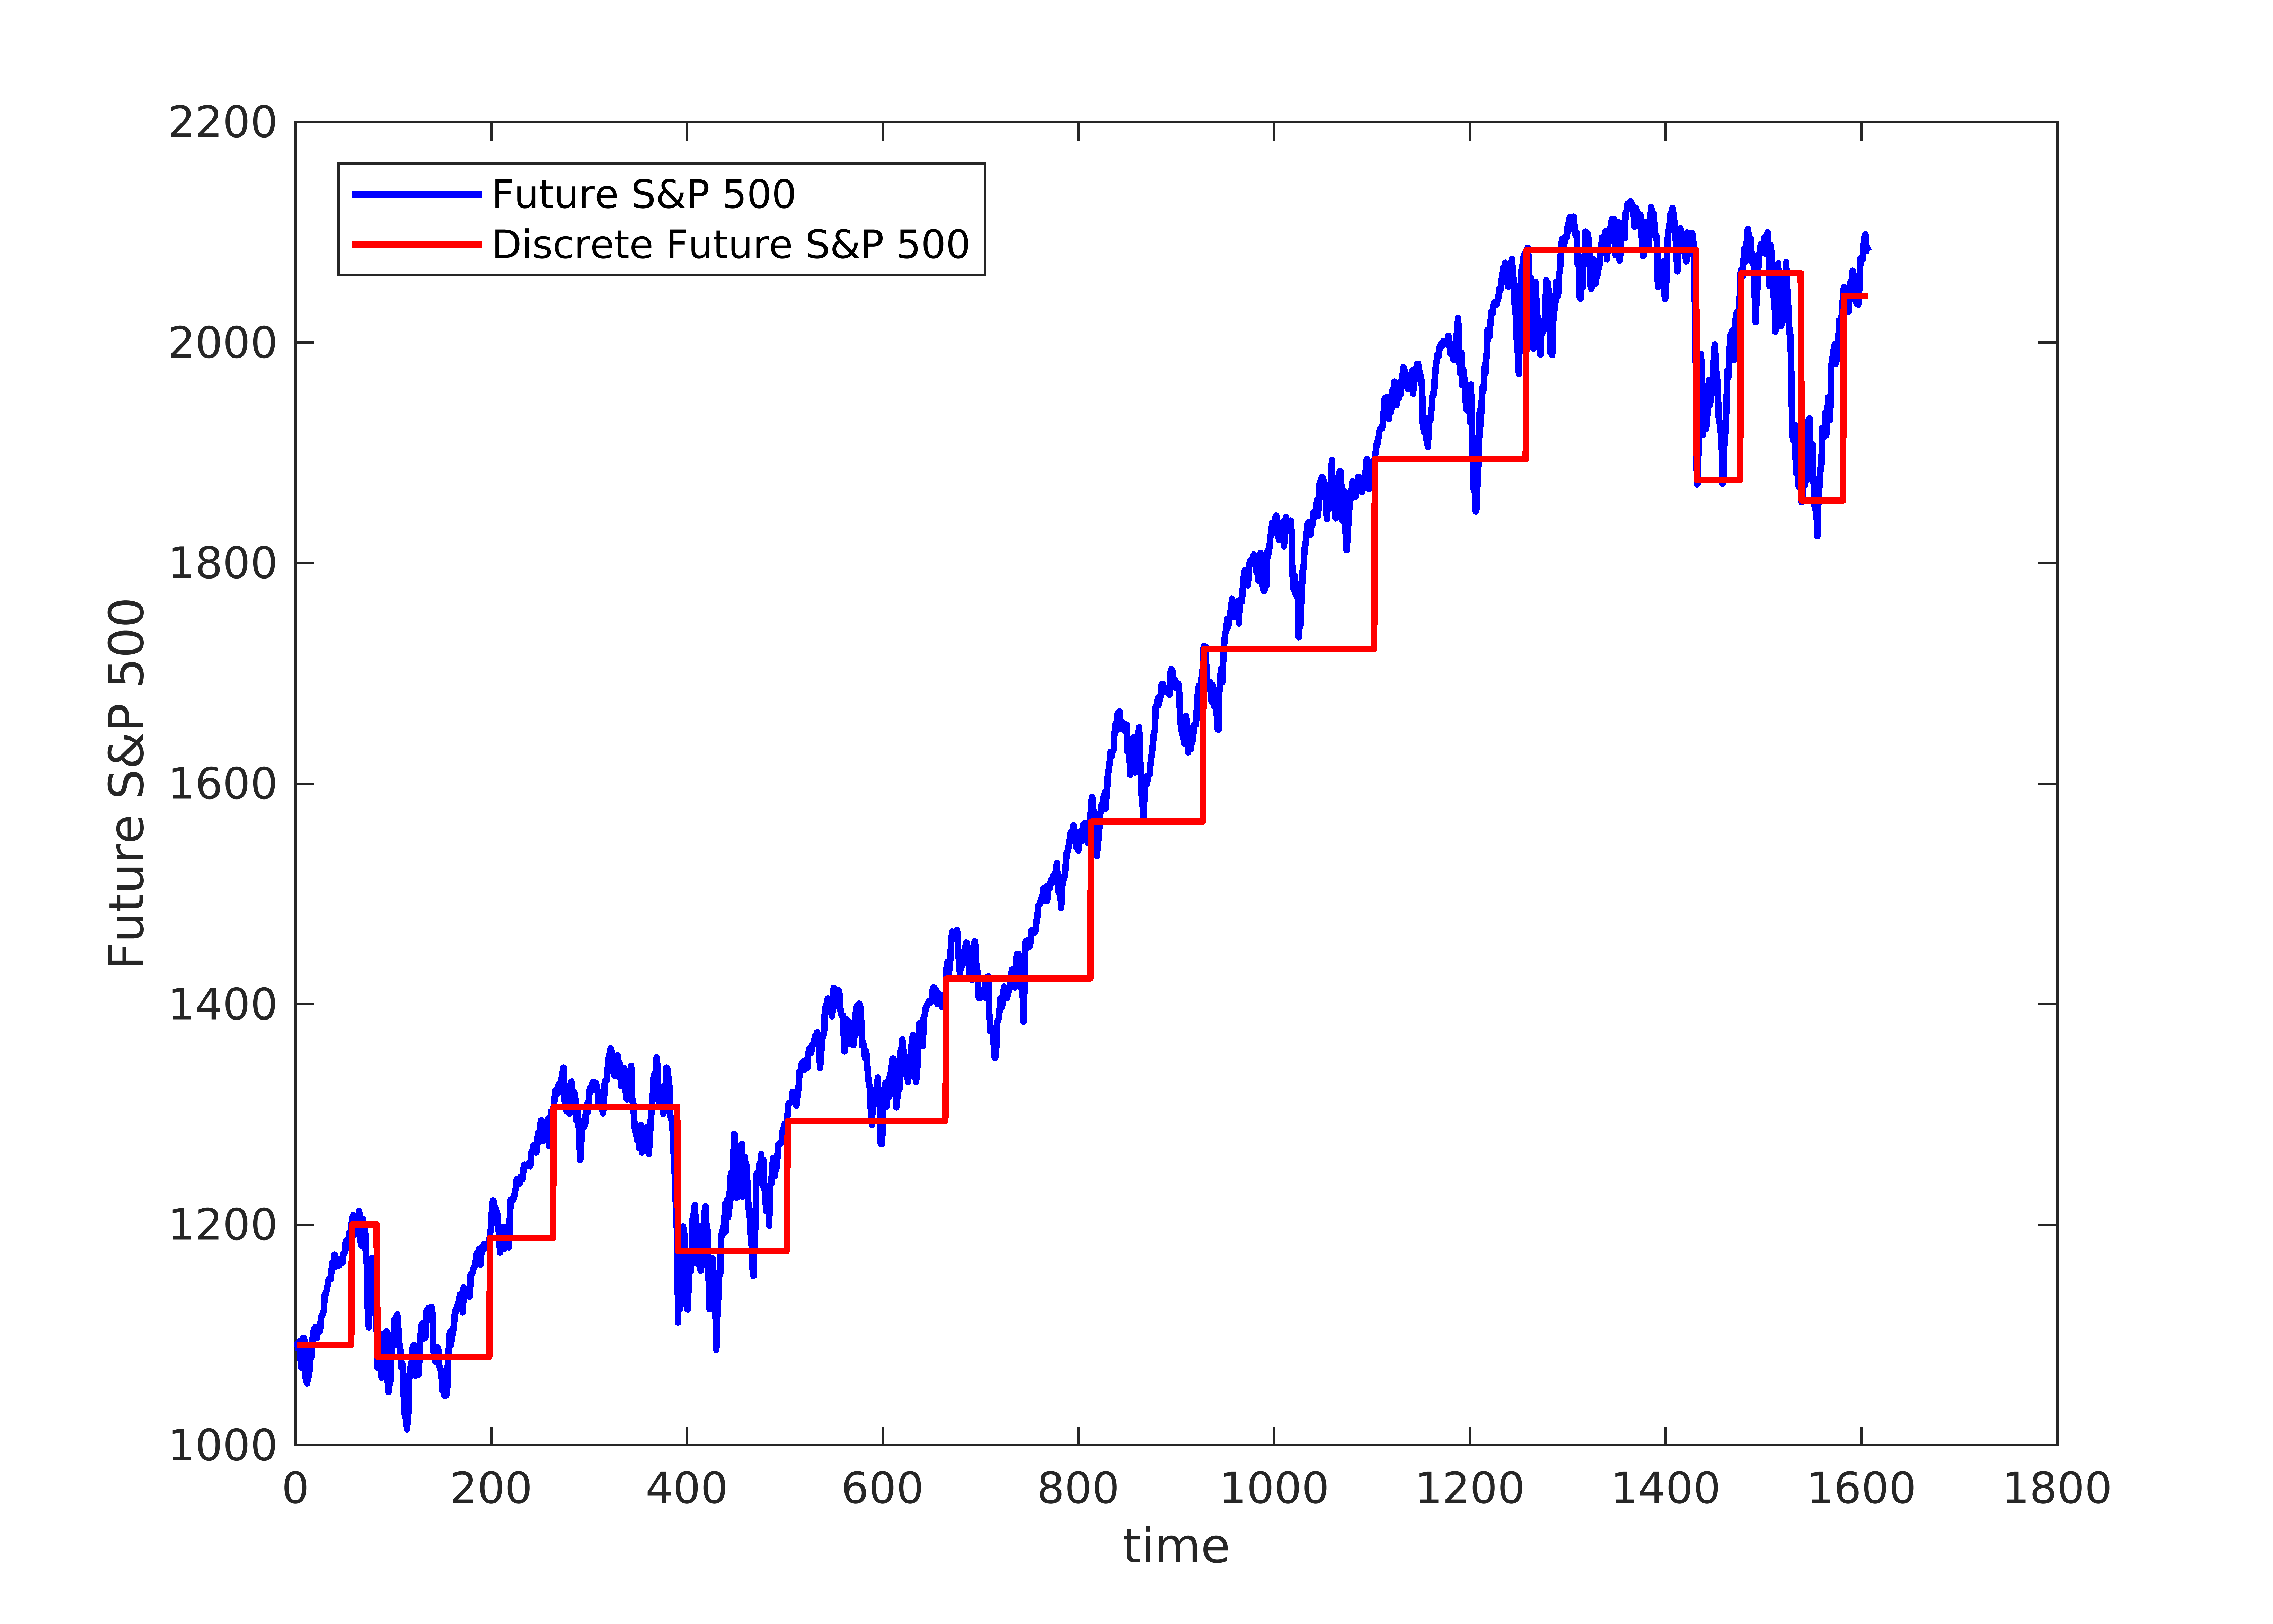
\includegraphics[width=1\linewidth]{Images/DiscreteDynamics}
			\end{figure}
		\end{column}
	\end{columns}
	\pause
	\begin{block}{Dinamica di Portafoglio}
		\begin{equation*}
		x_{k+1} = x_k(\exp\{r \tau_{k+1} \} + u_kJ\widetilde{N}_{k+1}), \quad k \in \mathbb{N}
		\end{equation*}
	\end{block}
	
\end{frame}






\begin{frame}{Mappe allocazione titolo rischioso}
	\begin{columns}
		\begin{column}{0.4\textwidth}
			\begin{block}{parametri investimento}
				\begin{itemize}
					\item 10 riallocazioni 
					\item $r=1\%$
					\item $X_{10} = [1.07^4,\infty]$
				\end{itemize}
			\end{block}
			\textbf{probabilità raggiungimento target}:
			$p^{\star}=73.5\%$
		\end{column}
		\begin{column}{0.6\textwidth}
			\begin{figure}
				\centering
				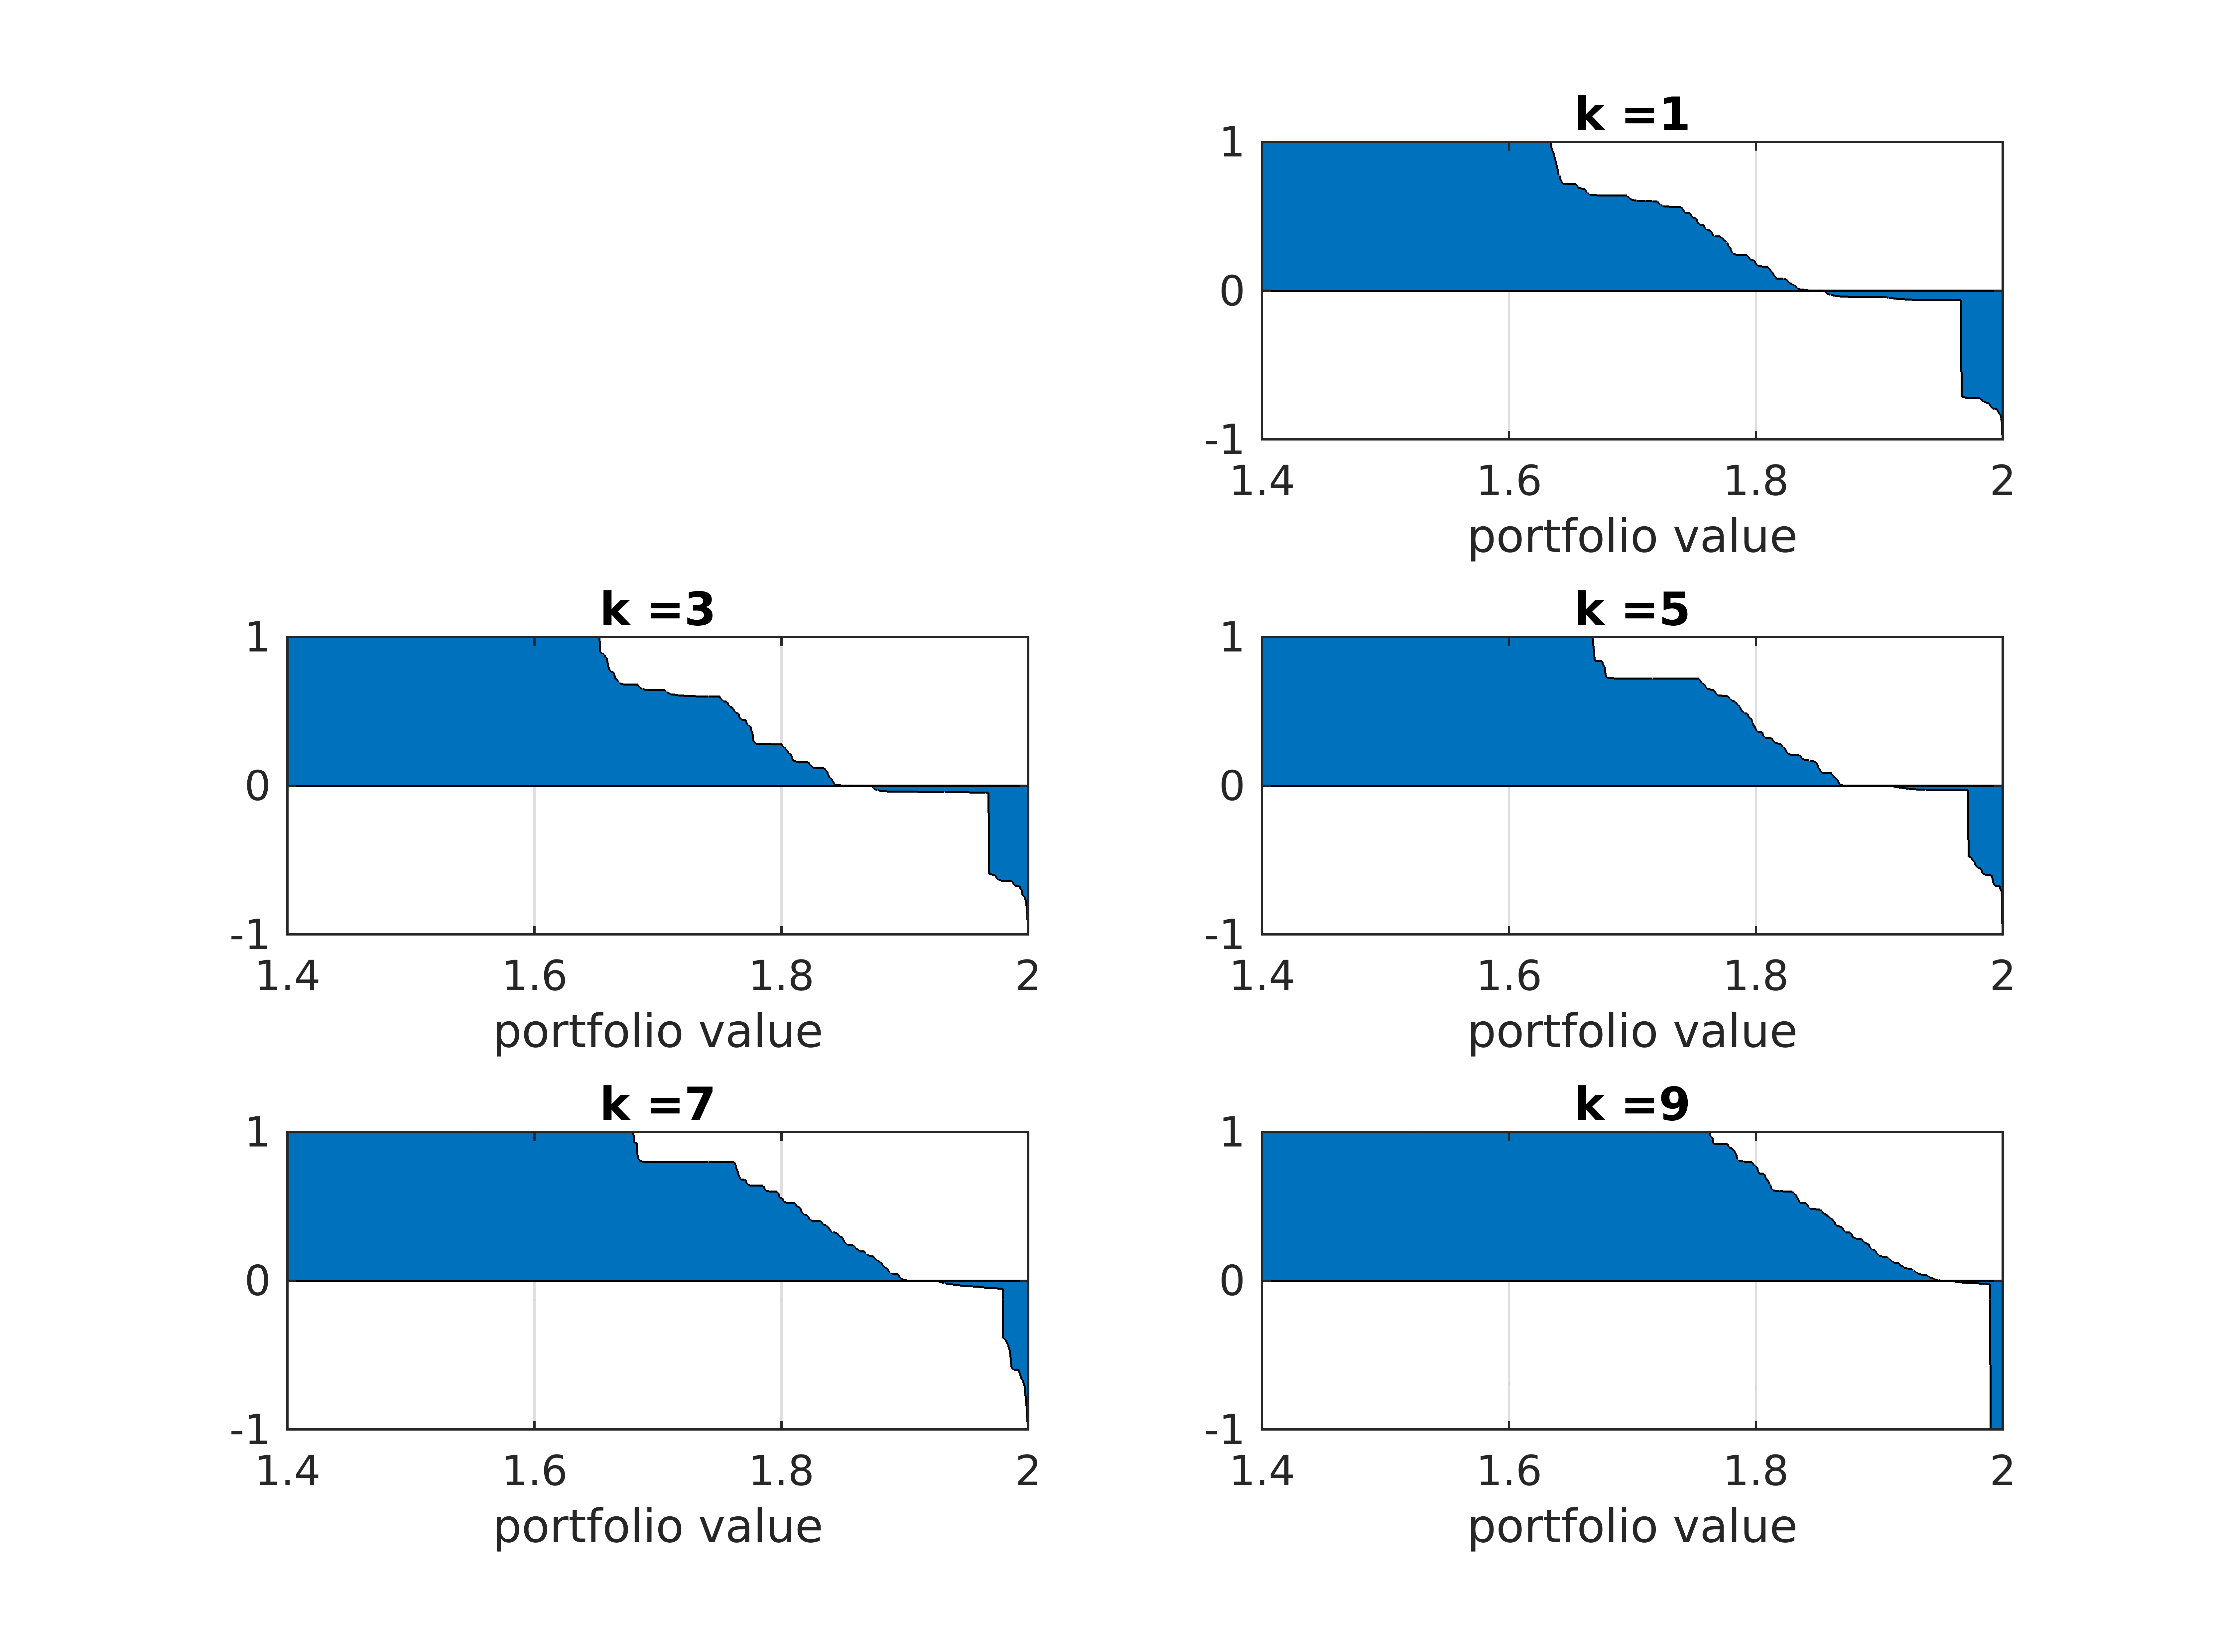
\includegraphics[width=1.1\linewidth]{Images/mapsbasic}
			\end{figure}
		\end{column}
	\end{columns}
\end{frame}

\begin{frame}{Estensione}
	
	
\end{frame}




